% CoRe paper skeleton (2026-10-01), on the PVLDB template in ../../pvldbstyle-master.
% Section plan and evidence: ../00-论文骨架.md. Numbers come from the rebuilt (v2) tables.
% PVLDB Vol. 20 (checked 10-03): single-blind (names and affiliations on page 1); 12 pages
% excluding references, appendices included; title suffix [Experiment, Analysis & Benchmark];
% link to the full reproducibility package required at the first submission.

\documentclass[sigconf, nonacm, balance=false]{acmart}
\usepackage{enumitem}
\usepackage{tabularx}
\setlist[itemize]{leftmargin=1.1em, itemsep=1pt, topsep=2pt, parsep=0pt}
\setlist[enumerate]{leftmargin=1.4em, itemsep=1pt, topsep=2pt, parsep=0pt}

\newcommand\vldbdoi{XX.XX/XXX.XX}
\newcommand\vldbpages{XXX-XXX}
\newcommand\vldbvolume{20}
\newcommand\vldbissue{1}
\newcommand\vldbyear{2027}
\newcommand\vldbauthors{\authors}
\newcommand\vldbtitle{\shorttitle}
\newcommand\vldbavailabilityurl{}
\newcommand\vldbpagestyle{plain}

\newcommand{\core}{\textsc{CoRe}}
\newcommand{\companion}{\href{../CoRe-companion-index.md}{companion materials}}
\newcommand{\todo}[1]{\textcolor{red}{[TODO: #1]}}
% Numbered finding at the end of each results section (cf. the "Finding" boxes of EA&B papers).
\newcounter{finding}
\newcommand{\finding}[1]{\par\smallskip\noindent\refstepcounter{finding}%
  \fcolorbox{black!55}{black!4}{\parbox{\dimexpr\columnwidth-2\fboxsep-2\fboxrule\relax}{\small\textbf{Finding~\thefinding.} #1}}%
  \par\smallskip}

% Many full-width floats (figures and tables): let up to three sit at the top of a page and keep
% LaTeX from stalling on deferred floats.
\setcounter{dbltopnumber}{3}
\renewcommand{\dbltopfraction}{0.85}
\extrafloats{40}
% Spacing around floats. sigconf sets \flushbottom with \parskip=0pt (no stretch), so the space
% left in a column that cannot break exactly at its bottom was spread over the only stretchable
% glue, the gaps around figures, tables and headings. With \raggedbottom that space stays at the
% bottom of the column and every float keeps the fixed gaps below (LaTeX defaults: 20pt
% float-to-text, 12pt between floats, 10pt between a float and its caption). Fonts and margins
% are left as in the template.
\raggedbottom
\setlength{\textfloatsep}{10pt plus 1pt minus 2pt}
\setlength{\dbltextfloatsep}{10pt plus 1pt minus 2pt}
\setlength{\floatsep}{8pt plus 1pt minus 2pt}
\setlength{\dblfloatsep}{8pt plus 1pt minus 2pt}
\setlength{\intextsep}{8pt plus 1pt minus 2pt}
\captionsetup{skip=5pt}

\begin{document}
\title{Cleaning or Recalling? Disentangling Memorization and World Knowledge in LLM-based Data Cleaning [Experiment, Analysis \& Benchmark]}

% Single-blind review: real names and affiliations, one \author block each.
\author{Jingru Yang}
\affiliation{\institution{Minzu University of China}}
\email{okiyang@muc.edu.cn}

\author{Zheng Chen}
\affiliation{\institution{Minzu University of China}}
\email{202301050@muc.edu.cn}

\author{Ju Fan}
\affiliation{\institution{Renmin University of China}}
\email{fanj@ruc.edu.cn}

\begin{abstract}
High scores on public data-cleaning benchmarks can reflect knowledge of familiar entities,
leaving unclear how well an LLM can repair unfamiliar data. We present \core{}, a controlled
evaluation protocol linking recovery evidence, assigned values and repair credit. It compares
benchmarks with fresh real records and name surrogates built from English words or syllables.
The paired surrogates retain
error positions and transfer error mechanisms, linking performance changes to the evidence
each error leaves available for repair. Across 21 controlled tables and eight LLMs, we find
large knowledge effects on Hospital's identity columns and on Movies for commercial models.
For example, DeepSeek-V4-Pro's Hospital identity-column repair F1 falls from 0.88 to 0.16
after syllable renaming. This advantage persists on fresh records, while a separate continuation
probe finds no positive evidence of benchmark-row memorization in the tested models.
Yet recovering a familiar fact is not always the task's goal: models replace assigned movie
directors with real-world credits, sometimes even under table-evidence instructions. Whether
an edit receives repair credit then depends on the reference. On Rayyan, checks against title-matched
PubMed records identify reference discrepancies, and 94\% of TabClean's credited repairs
reproduce the reference date transformation. These results connect the evidence supporting
a repair to the task's preservation requirements and the reference that awards credit.
\end{abstract}

\maketitle

%%% VLDB block start %%%
\pagestyle{\vldbpagestyle}
\begingroup\small\noindent\raggedright\textbf{PVLDB Reference Format:}\\
\vldbauthors. \vldbtitle. PVLDB, \vldbvolume(\vldbissue): \vldbpages, \vldbyear.\\
\href{https://doi.org/\vldbdoi}{doi:\vldbdoi}
\endgroup
\begingroup
\renewcommand\thefootnote{}\footnote{\noindent
This work is licensed under the Creative Commons BY-NC-ND 4.0 International License. Visit \url{https://creativecommons.org/licenses/by-nc-nd/4.0/} to view a copy of this license. For any use beyond those covered by this license, obtain permission by emailing \href{mailto:info@vldb.org}{info@vldb.org}. Copyright is held by the owner/author(s). Publication rights licensed to the VLDB Endowment. \\
\raggedright Proceedings of the VLDB Endowment, Vol. \vldbvolume, No. \vldbissue\ %
ISSN 2150-8097. \\
\href{https://doi.org/\vldbdoi}{doi:\vldbdoi} \\
}\addtocounter{footnote}{-1}\endgroup
%%% VLDB block end %%%

%%% VLDB block start %%%
\ifdefempty{\vldbavailabilityurl}{}{
\vspace{.3cm}
\begingroup\small\noindent\raggedright\textbf{PVLDB Artifact Availability:}\\
The statistical core, with construction and evaluation code, numerical witnesses and
benchmark-specific replay materials, is available at \url{\vldbavailabilityurl}.
\endgroup
}
%%% VLDB block end %%%


\section{Introduction}\label{sec:intro}
Data cleaning methods detect and repair erroneous values and are commonly evaluated on a small
set of public benchmark tables~\cite{rahm2000data,ilyas2019book,chu2016overview,abedjan2016detecting}.
Large language models (LLMs) have opened new approaches to data management~\cite{fernandez2023disrupt},
including few-shot error detection and imputation competitive with specialized
systems~\cite{narayan2022wrangle}. Recent cleaners use LLMs to edit values, derive rules or write
cleaning programs~\cite{ni2025zeroed,ni2024iterclean,zhang2025data,tabclean2026}. Their benchmark
scores, however, can draw on information beyond the table being cleaned.

Public cleaning benchmarks contain familiar hospitals, films, breweries and articles.
Pretrained models can retrieve entity facts from their parameters~\cite{petroni2019lama,mallen2023trust},
while public tabular datasets can carry signals of prior exposure~\cite{bordt2024elephants,silvestri2025knowtable}.
A correct repair can therefore combine benchmark-row memory, knowledge of the entity
(\emph{entity knowledge}), knowledge of English word forms (\emph{spelling knowledge}), and
evidence within the table. Scores on familiar entities need not predict repair quality
on unfamiliar data.

\smallskip\noindent\textbf{Example 1.1.} In Hospital, DeepSeek-V4-Pro repairs the corrupted
city \texttt{birminghxm} to \texttt{birmingham}. In a copy with fictitious syllable
names, the analogous corruption \texttt{hepmxrmxr} of \texttt{hepmormor} is left unchanged.
The table structure is the same, but the familiar city has disappeared. Other errors retain
useful recovery evidence after renaming. Movies, for example, gives some years as three-year
ranges, whose middle candidate usually matches the reference (Figure~\ref{fig:year}). A score
drop can thus reflect either the loss of a familiar value or a failure to use evidence that
remains in the input.\smallskip

Controlled tabular evaluations already test recognition and completion of dataset instances
(KnowTable~\cite{silvestri2025knowtable}) and adherence to counterfactual database values
(ContraTable~\cite{wang2026contratable}). Cleaning poses a further question: which input values
should change, and what makes a change count as a repair? Interpreting scores requires
connecting recovery evidence with the values to preserve and the reference used for scoring.

In this paper, we present \core{}, a protocol that compares repairs on dirty/reference pairs
under controlled entity replacements. Each benchmark is compared with \emph{fresh} real records,
a \emph{words surrogate} with fictitious English-word names, and a \emph{syllable surrogate}
with meaningless names. The original and its surrogates share rows and error positions, while
fresh records carry the same kinds of errors. Paired substitutions test entity familiarity
and word form. Fresh records test performance beyond the benchmark, while a separate
continuation probe tests for benchmark-row memory.

The constructions retain the original cleaning problems by transferring error mechanisms,
rather than adding arbitrary noise. This is particularly important for Movies, where errors
often reflect differences between two legitimate sources. Fictitious names must also hide the
entity without themselves looking erroneous. We build 21 controlled tables, with three
construction seeds for Hospital and Movies. Their surrogates contain about 41,000 fictitious
values, assessed by 506 acceptance checks. We evaluate four commercial and four open-weight
LLMs, alongside Baran~\cite{mahdavi2020baran} and the program-generating cleaner
TabClean~\cite{tabclean2026}, using about 23,000 prompts. Our main findings are as follows.

Familiar entities supply recovery evidence. On Hospital's \emph{identity columns},
which name or locate an entity, three commercial models lose 0.59 to 0.72 repair F1 after
replacement with syllable names. On Movies, the four commercial models have fresh--words gaps
of $+$0.17 to $+$0.42 at construction seed~0 (Table~\ref{tab:main}). Figure~\ref{fig:decomposition}
shows the pattern for DeepSeek-V4-Pro: Hospital and Movies surrogate scores fall sharply,
while fresh real records retain high scores.

\begin{figure}[tb]
  \centering
  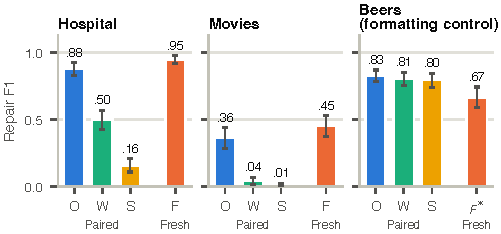
\includegraphics[width=\columnwidth]{figures/fig1_decomposition.pdf}
  \caption{DeepSeek-V4-Pro's repair F1 falls on Hospital and Movies surrogates. O/W/S share rows
  and error positions; F uses fresh real records. Results use Hospital/Movies identity columns
  and all Beers columns, with 95\% bootstrap intervals. $^{*}$Beers F is descriptive because brewery
  concentration and alcohol-content distributions differ; knowledge comparisons use the paired
  O/W/S conditions.}
  \label{fig:decomposition}
\end{figure}

The continuation probe finds no positive evidence of benchmark-row memorization in its tested
models (Section~\ref{sec:memorization}). The knowledge effects also persist across construction
seeds and, for DeepSeek-V4-Pro, with labeled examples and error positions. Within Qwen2.5,
Hospital's total effect grows across the three model sizes. Baran's whole-table and TabClean's
results vary little across entity replacements, illustrating how table redundancy and
formatting rules supply other repair evidence (Sections~\ref{sec:knowledge}--\ref{sec:generalize}).

Yet a familiar fact can be the wrong value to preserve. Commercial models rewrite
68\%--100\% of assigned directors of known films toward real-world credits. Table-evidence
instructions reduce these rates unevenly, while hospital and brewery city rewrites are
less frequent (Section~\ref{sec:conflict}).

The reference then determines repair credit. Rayyan contains systematic date and page
conversions (Section~\ref{sec:quality}). Stratified field checks against title-matched PubMed records yield a weighted
reference-check failure rate of 95.2\% (95\% interval: 91.2--97.8\%), using the audit input's
948-cell error-type composition. On TabClean's input version, 434 of 461 credited repairs
(94\%), after excluding development rows, reproduce the reference date transformation.

\noindent We make the following contributions:
\begin{itemize}
  \item We propose \core{}, a controlled evaluation protocol that transfers benchmark errors
  to paired name surrogates and relates repair scores to the recovery evidence retained in
  the input (Section~\ref{sec:protocol}).
  \item We construct controlled tables for three benchmarks and provide construction and
  evaluation code, numerical witnesses and replay materials. Public statistical replay
  and authorized local validation provide distinct verification entries
  (Sections~\ref{sec:construction} and~\ref{sec:artifact}).
  \item We characterize both knowledge-dependent repair and directed rewriting of assigned
  values across eight LLMs, with separate continuation and information-condition checks
  (Sections~\ref{sec:memorization}--\ref{sec:conflict}).
  \item We identify systematic reference transformations in Rayyan and trace how they receive
  repair credit (Section~\ref{sec:quality}).
\end{itemize}

Section~\ref{sec:related} provides background and related work.
Sections~\ref{sec:protocol}--\ref{sec:setup} describe the protocol, constructions and evaluation
settings. Sections~\ref{sec:memorization}--\ref{sec:quality} present the analyses, followed by
recommendations and limitations in Section~\ref{sec:discussion}.

\section{Background and Related Work}\label{sec:related}

\subsection{Cleaning Benchmarks}\label{sec:benchmarks}

Cleaning systems draw on several kinds of evidence. Rules repair constraint violations or
apply fixing patterns~\cite{dallachiesa2013nadeef,chu2013holistic,wang2014fixing}, while KATARA
uses knowledge bases and crowdsourcing~\cite{chu2015katara}. Learned detectors use a small
set of labels~\cite{mahdavi2019raha,heidari2019holodetect,neutatz2019ed2}; Baran learns context
models for repair~\cite{mahdavi2020baran}, and HoloClean combines signals through probabilistic
inference~\cite{rekatsinas2017holoclean}. Experimental studies compare detection and repair
tools~\cite{abedjan2016detecting,ni2024repair} and their effects on machine-learning
models~\cite{li2021cleanml,abdelaal2023rein}. ActiveClean integrates progressive cleaning with
statistical model training~\cite{krishnan2016activeclean}. BART controls detectability and
repairability during error generation~\cite{arocena2015bart}.

We select public dirty/reference pairs from Raha and Baran for their complementary error
profiles (Table~\ref{tab:datasets}). Hospital's damaged names contrast with Movies' source-specific
mappings and retained candidates. Beers adds a formatting contrast: its errors retain the
information needed for repair. Rayyan's spreadsheet
transformations instead expose what reference matching rewards. For cleaning we use 1,000-row
tables, with Movies and Beers drawn as subsets of the full tables. Flights and Tax serve only
the continuation probe.

\begin{table*}[t]
  \caption{Benchmarks distributed with Raha and Baran. Parentheses give identity-column error
  cells. CMS: US Centers for Medicare \& Medicaid Services.}
  \label{tab:datasets}
  \small
  \setlength{\tabcolsep}{4pt}
  \begin{tabular*}{\textwidth}{@{\extracolsep{\fill}}lllrll@{}}
    \toprule
    Dataset & Entities & Source & Error cells & Kind of error & Use in this paper \\
    \midrule
    Hospital & US hospitals & CMS registry & 509 (219) & one character replaced by \texttt{x} & four conditions \\
    Movies & films & IMDb and Rotten Tomatoes & 1,965 (379) & the other source's value; formatting rules & four conditions \\
    Beers & craft beers and breweries & CraftCans.com & 565 (127) & state glued to city; alcohol \% suffix & formatting control \\
    Rayyan & biomedical articles & PubMed & 948 & spreadsheet conversions (Section~\ref{sec:quality}) & quality analysis \\
    Flights & flight times & 38 web sources & \multicolumn{2}{l}{not used for cleaning} & memorization probe \\
    Tax & personal tax records & --- & \multicolumn{2}{l}{not used for cleaning} & memorization probe \\
    \bottomrule
  \end{tabular*}
\end{table*}

\emph{Identity columns} name or locate an entity: provider number, name, address, city, ZIP code,
county and phone in Hospital; identifier, title, director, writers and actors in Movies; and beer,
brewery and city in Beers. We distinguish their recovery from repairs of other values, such as
film years and formatting errors.

\subsection{LLM-Based Cleaners}\label{sec:cleaners}

Few-shot prompting can match specialized systems on studied detection, imputation and matching
tasks~\cite{narayan2022wrangle}. Subsequent work includes table-tuned and preprocessing
models~\cite{li2024tablegpt,zhang2024jellyfish} and entity
matchers~\cite{tu2023unicorn,peeters2025entity}. LLM cleaners label errors
(ZeroED~\cite{ni2025zeroed}), iterate on repairs (IterClean~\cite{ni2024iterclean}), derive
ontological or semantic rules (LLMClean~\cite{10.1007/978-3-031-70421-5_7},
Cocoon~\cite{zhang2025data}), standardize data as agents (CleanAgent~\cite{qi2024cleanagent}),
compile curation pipelines (SEED~\cite{chen2024seeddomainspecificdatacuration}), or generate
cleaning programs (TabClean~\cite{tabclean2026}). We study direct value editing and generated
programs under controlled entity replacements.

\subsection{Related Work}\label{sec:relatedwork}

\textbf{LLMs on enterprise data.} Enterprise annotation and integration studies examine domain
context, schemas, table width and sparsity~\cite{kayali_cidr25,demiralp2024enterprise}.
Bodensohn et al. also observe a bias toward familiar SQL despite explicit SIGNAL
documentation~\cite{bodensohn2025enterprise}. \core{} compares repair and preservation
under controlled entity replacements.

\textbf{Memorization and contamination.} LLMs can memorize training text, with stronger effects
as models grow or data repeat~\cite{274574,carlini2023quantifying}. Detection methods include
benchmark completion~\cite{ICLR2024_bc39a59c}, likelihoods of canonical and shuffled orderings
under exchangeability~\cite{oren2024proving}, and least-likely token
probabilities~\cite{shi2024detecting}. Benchmark-specific records and surveys document these
issues~\cite{sainz2023trouble,xu2024contamination}, while mitigation restricts exposure or
refreshes questions~\cite{jacovi2023stop,white2025livebench}.
For tables, Bordt et al.~\cite{bordt2024elephants} find strong memorization of Iris and Wine;
Adult's signals concentrate in headers and initial rows. KnowTable~\cite{silvestri2025knowtable}
compares completion and existence queries over real, column-resampled, swapped and obfuscated
variants, with non-neural baselines and statistical tests. Our comparison instead follows
dirty/reference cell pairs: we transfer their error mechanisms to renamed entities and relate
repair scores to the candidates and patterns left in the input. The continuation probe separately
uses structural baselines to distinguish predictable cells from evidence of row memory.

\textbf{Knowledge and counterfactual evaluation.} Models store facts about entities, especially
popular ones~\cite{petroni2019lama,mallen2023trust,3618408.3619049}. Entity substitutions in QA
reveal conflicts between parametric and contextual answers~\cite{longpre2021conflicts,xie2024adaptive,xu2024conflictsurvey},
and counterfactual or low-probability variants expose dependence on familiar task
instances~\cite{wu2024reasoning,mccoy2024embers,ICLR2025_ec2e7a89}. DisentQA separates contextual
and parametric answers~\cite{neeman2023disentqa}. In data management,
ContraTable~\cite{wang2026contratable} pairs original and counterfactual databases to compare
answer faithfulness across lookup, joins and temporal reasoning. A cleaner must both change
errors and preserve assigned values. Our conflict test measures directed rewrites of
reference-consistent cells toward familiar facts, alongside arbitrary edits
(Section~\ref{sec:conflictmetric}). Fictional ontologies and pseudowords also limit factual shortcuts
in reasoning tasks~\cite{saparov2023language,derelab2026}. We contrast word and syllable names
for cleaning.

\textbf{Benchmark quality.} Label errors can change model comparisons, particularly on
mislabeled subsets and at higher error prevalence~\cite{northcutt2021pervasive}. Spreadsheet
conversion can also silently alter values~\cite{ziemann2016gene}. Rayyan lets us trace credited
repairs back to reference transformations and examine what the score rewards.

\section{The \core{} Protocol}\label{sec:protocol}

\core{} compares a cleaner on controlled versions of a benchmark's dirty/reference table pair
(Figure~\ref{fig:overview}). The cleaner sees dirty values, with its prompt, information access
and scoring held fixed within a setting. Paired surrogates test dependence on familiar entities
and word forms; fresh real records test whether high scores persist outside the original
benchmark. Separate conflict and reference checks ask which values should be preserved and
which edits receive repair credit (Sections~\ref{sec:conflict} and~\ref{sec:quality}).

\begin{figure*}[t]
  \centering
  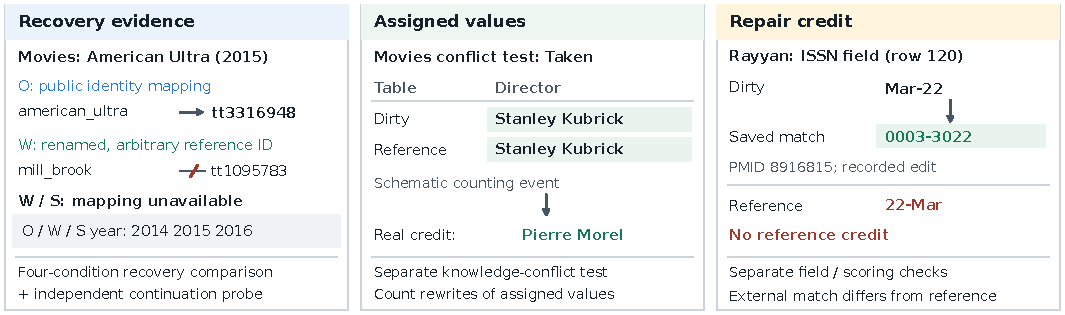
\includegraphics[width=\textwidth]{figures/fig0_overview.pdf}
  \caption{\core{} transfers errors to paired name surrogates and fresh real records. Recovery
  contrasts motivate questions about assigned-value preservation and Rayyan repair credit.
  Hospital city tokens illustrate error transfer; the continuation probe tests row memory.}
  \label{fig:overview}
\end{figure*}

\subsection{Four Conditions and Their Comparisons}\label{sec:conditions}

Besides the original (\textbf{O}), \core{} builds three tables with the same schema and size:
\begin{itemize}
  \item \textbf{Fresh (F)} uses real records outside the benchmark: newer registry records for
  Hospital, or other films and beers. Their entities may remain familiar to a model.
  \item \textbf{Words surrogate (W)} replaces identity values one to one with fictitious names
  made of English words and random numeric identifiers. Non-identity values and error positions
  stay fixed.
  \item \textbf{Syllable surrogate (S)} uses syllable names in the same construction, retaining
  generic terms such as \emph{hospital} and \emph{street}.
\end{itemize}
Table~\ref{tab:example} illustrates the four conditions on Hospital rows.

\begin{table*}[t]
  \caption{Hospital identity fields across conditions, with the corrupted city in bold.
  O/W/S share a row and error position. $^*$F draws a newer registry row with updated quality
  measures, rather than a row-paired replacement of O.}
  \label{tab:example}
  \small
  \begin{tabular*}{\textwidth}{@{\extracolsep{\fill}}lllllr@{}}
    \toprule
    & Name & Address & City & County & Phone \\
    \midrule
    O & callahan eye foundation hospital & 1720 university blvd & \textbf{birminghxm} & jefferson & 2053258100 \\
    F$^*$ & southeast health medical center & 1108 ross clark circle & \textbf{dxthan} & houston & 3347938701 \\
    W & timber hollow regional hospital & 5749 glen road & \textbf{xill pine} & sunset prairie & 6175712390 \\
    S & vasrhokel regional hospital & 8928 zarquen street & \textbf{hepmxrmxr} & lotorcal & 6061657772 \\
    \bottomrule
  \end{tabular*}
\end{table*}


\begin{table*}[t]
  \caption{Condition contrasts and their interpretation. O/W/S pair rows, error cells, chunks
  and non-identity values; F shares schema, size and error recipes or rules.}
  \label{tab:conditions}
  \small
  \begin{tabularx}{\textwidth}{@{}l >{\raggedright\arraybackslash}X@{}}
    \toprule
    Contrast & Interpretation and comparison assumption \\
    \midrule
    O$-$W & Paired entity-familiarity contrast; its magnitude also depends on the change from real names to English-word combinations. \\
    W$-$S & Spelling contrast; interpretation depends on the difficulty of the two naming styles and any regularities they introduce. \\
    O$-$S & Total knowledge effect under entity replacement, combining changes in entity familiarity and word form. \\
    F$-$W & Fresh--words comparison; entity familiarity changes with record difficulty and, where recipes cannot transfer exactly, error composition. \\
    O$-$F & Original--fresh comparison; benchmark exposure and table difficulty both change. Memorization is tested separately. \\
    \bottomrule
  \end{tabularx}
\end{table*}

Let $s_O,s_F,s_W,s_S$ denote a method's repair F1 in a fixed column group.
Table~\ref{tab:conditions} defines three paired contrasts: O\,$-$\,W, W\,$-$\,S and O\,$-$\,S.
They measure score changes under entity and word-form replacement; the first two sum to the third. Their interpretation
uses the error profiles and method controls, since renaming changes candidate values and
construction regularities as well as familiarity. We report F\,$-$\,W separately to examine
knowledge effects on fresh records; it is not a component of O\,$-$\,S. O\,$-$\,F combines
exposure and difficulty, so it supports the independent continuation probe rather than defining
a pure memory effect.

\subsection{What Makes an Error Recoverable?}\label{sec:recoverability}

A fictitious Rotten Tomatoes slug does not determine its randomly assigned IMDb identifier,
whereas a film-year range retains the same candidate years after renaming. These errors
motivate three recovery cases
(Table~\ref{tab:recoverability}): \emph{locally reversible} errors retain the information for a
format conversion once its target convention is established (R1); \emph{constrained} errors
retain candidates or useful regularities (R2); and \emph{underdetermined} errors need an external
fact, additional records or a source choice absent from the shown chunk (R3). A column may
contain several cases, and additional examples or records can change a cell's recoverability.

These profiles contrast available recovery evidence with missing mappings. The S score measures
residual repair after renaming, including local rules and construction regularities.

\begin{table}[t]
  \caption{Recovery evidence available in the shown input, under the cases defined in
  Section~\ref{sec:recoverability}.}
  \label{tab:recoverability}
  \small
  \begin{tabularx}{\columnwidth}{@{}>{\raggedright\arraybackslash}p{0.25\columnwidth} >{\raggedright\arraybackslash}X@{}}
    \toprule
    Case & Examples in the benchmark conditions \\
    \midrule
    R1: locally reversible & Beers city/state split and percentage suffix; Movies thousands separators and integer ratings with an added \texttt{.0}. \\
    R2: constrained & Movies year ranges; Hospital name typos with a matching candidate; syllable names with a restricted construction vocabulary. \\
    R3: underdetermined & Random fictitious identifiers; omitted film credits; source-specific ratings and durations not recoverable from the other source. \\
    \bottomrule
  \end{tabularx}
\end{table}

\subsection{Chunking, Prompting and Scoring}\label{sec:scoring}

The main input contains 20 rows from different entities, preventing copying from another record
of the same hospital or brewery while retaining cross-entity patterns. The same entity grouping
gives O/W/S identical chunks, 50 per table. A zero-shot prompt asks for erroneous cells and
correct values in JSON and asks the cleaner to leave correct cells unchanged. Other information
settings are defined in Section~\ref{sec:setup}.

Let $E$ be the cells whose dirty and reference strings differ, $P$ the cells effectively edited
after no-ops are removed, and $R \subseteq P \cap E$ those set to the reference value. Then
\begin{equation*}
  \textit{prec} = \frac{|R|}{|P|}, \qquad \textit{rec} = \frac{|R|}{|E|}, \qquad
  F1 = \frac{2 \cdot \textit{prec} \cdot \textit{rec}}{\textit{prec} + \textit{rec}},
\end{equation*}
and detection F1 uses $P \cap E$ in place of $R$. Edit and repaired-value comparisons ignore
case and normalize whitespace, while $E$ uses original strings. Thus Movies' five case-only
title errors remain in $E$ but cannot earn repair credit. Identity columns are reported
separately from the others. The \companion{} specify normalization, reply handling and the
construction recipes used below.

\section{Building the Controlled Tables}\label{sec:construction}

The controlled tables retain the benchmark's error mechanisms while varying entities and word
forms. Error generators can vary detectability and repairability~\cite{arocena2015bart}; here,
we start from the observed error profile and transfer it to renamed values or fresh records.
Surrogates preserve non-identity cells and error positions, whereas fresh error counts depend
on whether recipes and rules apply to the new records. Naming rules keep fictitious values
from revealing identities or looking malformed. Table~\ref{tab:construction}
summarizes the constructions, with full recipes and checks in the \companion{}.

\begin{table*}[t]
  \caption{Controlled-table sources and scale. Error counts in parentheses are identity cells;
  values renamed are distinct one-to-one replacements. Seeds cover F, W and S.}
  \label{tab:construction}
  \small
  \begin{tabular*}{\textwidth}{@{\extracolsep{\fill}}l lr llr rc@{}}
    \toprule
    & \multicolumn{2}{c}{Original (O)} & \multicolumn{3}{c}{Fresh (F)} & \multicolumn{1}{c}{W and S} & \\
    \cmidrule(lr){2-3}\cmidrule(lr){4-6}\cmidrule(lr){7-7}
    Dataset & Entities & Errors & Source & Entities & Errors & Values renamed & Seeds \\
    \midrule
    Hospital & 45 hospitals & 509 (219) & CMS registry, July 2026 release & 34 hospitals (33 also in O) & 509 (219) & 296 & 3 \\
    Movies & 1,000 films & 1,965 (379) & IMDb datasets, Sept.\ 2026 & 1,000 films & 2,195 (371) & 6,018 & 3 \\
    Beers & 421 breweries & 565 (127) & Wikidata, Sept.\ 2026 & 94 breweries & 565 (127) & 1,712 & 1 \\
    \bottomrule
  \end{tabular*}
\end{table*}


\subsection{Hospital}\label{sec:build-hospital}

Hospital's characteristic corruption replaces a character by \texttt{x}: 508 of 509 error cells
follow this form, usually replacing every occurrence of that character. F uses the July 2026
CMS registry in the benchmark schema. Its 34 hospitals include 33 from O, but all quality
measures have changed, giving new rows about largely the same entities. We retain the original
per-column error counts and position-weighted substitution rule, with newly drawn error locations.

Surrogates rename each distinct identity value consistently and transfer the original errors
by position (Figure~\ref{fig:overview}). S uses an inventory of 24 syllables; W uses English-word
combinations. Generic suffixes preserve column conventions, and numeric identifiers become
random digits. The restricted syllable inventory supplies a recoverable regularity examined
in Section~\ref{sec:commercial}.

\subsection{Movies}\label{sec:build-movies}

Movies joins IMDb and Rotten Tomatoes records. Its 190 source-replaced rows, together with two
formatting rules, produce the errors in Table~\ref{tab:movieserrors}. A film can have a Rotten
Tomatoes slug instead of an IMDb identifier, a year range instead of a year, or credits that
add or omit people. For example, \emph{American Ultra} has \texttt{american\_ultra} in place of
\texttt{tt3316948}. Such differences require recovering the benchmark's preferred source value,
rather than merely fixing spelling.

\begin{table*}[t]
  \caption{Movies' 1,965 errors and their transfer mechanisms. Source-style errors occupy
  190 rows, with formatting rules also applied table-wide. Copied errors transfer cell recipes;
  drawn errors follow measured rates. Slugs are the film identifiers used in Rotten Tomatoes URLs.}
  \label{tab:movieserrors}
  \small
  \begin{tabular}{@{}lr p{6.4cm} p{3.75cm} p{3.75cm}@{}}
    \toprule
    Column & Errors & In the original & Fresh table & Surrogates \\
    \midrule
    identifier & 190 & Rotten Tomatoes slug (135 plain, 28 numbered, 27 with the year) & slug of the fresh title, forms at the original's rates & slug of the dirty fictitious title, same form \\
    year & 190 & range ``Y$-$1 Y Y$+$1'' & same range & the original's cell \\
    title & 17 & 12 edit recipes (capitalization, \& for \emph{and}, accent, punctuation, subtitle, article) & the same edits on a fresh title & the same edits on the fictitious title \\
    director & 43 & 115 names added, 1 dropped, 17 respelled & copied name by name & copied name by name \\
    writers & 129 & 123 names added, 51 dropped, 20 respelled; 5 cells emptied & copied name by name & copied name by name \\
    duration & 187 & Rotten Tomatoes format (105) or empty (80) & drawn at the original's rates & the original's cell \\
    rating & 261 & score pair (165) or empty (22); ``.0'' added (74) & drawn at the original's rates & the original's cell \\
    rating count & 768 & thousands separators on every count $\geq$ 1,000 & the same rule & the original's cell \\
    genre & 180 & Rotten Tomatoes genre vocabulary & copied slot by slot & the original's cell \\
    \bottomrule
  \end{tabular}
\end{table*}


F matches each original film to another feature film in the September 2026 IMDb snapshot,
using the same release year (or within two years) and the nearest logarithmic vote count among
eligible films with at least 1,000 votes. The corresponding 190 rows receive source-style errors.
People and title errors are transferred as recipes over names and edits; genre errors retain
the other source's vocabulary. A recipe that cannot apply to its assigned cell is moved to
another source-style row able to take it.

Some recipes remain inapplicable: four director and four writer errors stay clean, leaving 371
identity errors in F versus 379 in O/W/S. Formatting rules also change counts: the separator
rule affects all 1,000 fresh rating counts, compared with 768 in O. F therefore has 2,195 errors
at seed~0 versus 1,965 in O/W/S. These are fresh-record comparisons under transferred mechanisms,
with the non-paired interpretation defined in Table~\ref{tab:conditions}.

Surrogates rename the 6,018 distinct identity values one to one. Titles require special care:
retaining a real title's function words, numbers and punctuation can reveal the film. We
generate title shapes independently at the original's aggregate rates, exclude real title
words from W, and require generated titles to support their transferred edit recipes. Fictitious
IMDb identifiers and slugs are then formed consistently with those titles.

Recovery evidence varies even within a column. Of 105 duration errors expressed in hours and
minutes, unit conversion agrees with the reference in 50 and disagrees in 55. A locally available
conversion can therefore differ from the preferred source value. Year ranges instead retain
useful candidates, whose use we examine in Section~\ref{sec:knowledge}.

\subsection{Beers}\label{sec:build-beers}

All Beers errors retain the information needed for formatting repair. They append a percentage
sign to a fractional alcohol value, or glue a state to a city and empty the state field. Removing
the suffix or splitting the location restores the benchmark's convention. F uses 1,000 beers
from 94 Wikidata breweries~\cite{vrandecic2014wikidata}, excluding original beers and transferring
the original error forms and counts.

Surrogates preserve generic terms and consistent relationships between brewery and city names.
A one-word city stays one word, since a two-word fictitious city could resemble the city/state
error itself. These choices keep the naming transformation from introducing the formatting
problem the model is asked to solve.

\subsection{Acceptance Checks and Construction Seeds}\label{sec:acceptance}\label{sec:naming}

Acceptance checks cover structure, error kinds and counts, error strength, naming leakage,
fresh-source requirements and deterministic rebuilding. They distinguish fixed surrogate error positions from fresh-table
recipes and check that fictitious names neither identify real entities nor look erroneous.
The experimental tables pass 505 of 506 checks. Hospital W at seed~0 exceeds the error-strength
tolerance by a maximum gap of 10.5 percentage points against an eight-point tolerance; its error
positions remain unchanged. Full check details and thresholds are in the \companion{}.

Naming and leakage account for 263 of the 506 checks: one-to-one replacements,
exclusion of real values, and title-shape comparisons against chance-level matching.
Deterministic rebuilding verifies that the same rules yield identical tables,
separating implementation variation from variation across construction seeds.

Hospital and Movies have three construction seeds. Surrogates redraw names and applicable error
variants; F keeps its clean records and redraws errors. Seed ranges thus measure sensitivity
to naming and error draws, while bootstrap intervals summarize chunks of one construction.
Main tables report seed~0. Construction ranges appear in Table~\ref{tab:seeds}.

\section{Experimental Setup}\label{sec:setup}

\textbf{Models.} DeepSeek-V4-Pro~\cite{deepseekai2026deepseekv4} and
Qwen3.8-Max~\cite{qwen38} run with thinking disabled. GLM-5.3~\cite{zai2026glm53} retains
thinking at reasoning effort \emph{low}; GPT-6.1-Sol~\cite{openai2026gpt61sol} also uses
\emph{low}. Our client leaves GPT sampling parameters at API defaults, while the other runs
request temperature 0. Locally, vLLM~\cite{kwon2023vllm} uses greedy decoding for
the Qwen2.5 Instruct models at 7B, 14B and 32B (AWQ)~\cite{qwen2025qwen25}, and
Llama-3.1-8B-Instruct~\cite{dubey2024llama3}. OLMo-2-7B's instruction and base
variants~\cite{olmo2024olmo2} are auxiliary continuation models with a public pretraining corpus.
Replies still truncated after budget retries count as no corrections, including 8 of GLM-5.3's
500 Movies chunks. The \companion{} give token budgets and historical request settings.

\textbf{Methods and information.} The \emph{aligned} setting adds 20 labeled dirty/clean tuples
and error positions to the main chunks. Baran~\cite{mahdavi2020baran} receives the same information,
with three seeded runs, and also runs on whole tables with perfect detection or
Raha~\cite{mahdavi2019raha}. We disable Baran's Wikipedia-revision value models and Raha's
knowledge-base detector. TabClean uses DeepSeek-V4-Pro on whole tables, with its 150 labeled
development rows excluded from scoring. These settings distinguish information available within
a chunk from evidence supplied by repeated records and labels.

\textbf{Scale.} The study includes about 23,000 prompts for cleaning, aligned comparisons,
knowledge conflicts and continuation. Their breakdown and run specifications are in the
\companion{}. Table~\ref{tab:datasets} gives the dataset roles; the Rayyan analysis uses the
version-specific inputs defined in Section~\ref{sec:quality}.

\textbf{Statistics.} Condition differences use a chunk-level bootstrap~\cite{efron1993bootstrap}
with 2,000 resamples, paired for O/W/S, and 95\% percentile intervals. Each table's differences
form a family, with significance at Holm-corrected~\cite{holm1979simple} $p<0.05$. Near-zero
scores also use repaired-cell counts and paired-chunk sign tests, corrected over models.
Main tables show construction seed~0; seed ranges describe the variation defined in
Section~\ref{sec:acceptance}.

Conflict intervals resample entity means 2,000 times under the metric in
Section~\ref{sec:conflictmetric}, conditioning on the selected entities in fixed table contexts.
Rayyan intervals use 5,000 within-stratum resamples of saved binary checks, with fixed type
weights, conditioning on the selected title matches and field criteria
(Section~\ref{sec:rayyan-audit}). Both report 95\% percentile intervals.

\section{Testing Benchmark Memorization}\label{sec:memorization}

We test benchmark-row memorization with DeepSeek-V4-Pro, the four open-weight cleaners and
the instruction/base OLMo-2 variants. The probe asks a model to continue a table from a header
and ten consecutive rows, and tests whether dirty context elicits a clean reference value.
The \companion{} give the trial counts and clean/dirty and dataset-name settings.

\textbf{Separating structure from row memory.} Many next-row values are predictable from
repeated values and fixed record order. On Hospital, naive scoring gives DeepSeek-V4-Pro 47\%
continuation accuracy on cells absent from the context. We instead score \emph{hard} cells,
whose values are absent from the context column and not guessed by a column-mode or
most-frequent-successor baseline, both fitted leave-one-out. Accuracy then falls to 2.4\%.
The baselines control for structural predictability.

No tested model exceeds 0.085 on hard cells (Table~\ref{tab:p1}). DeepSeek's highest rates come
from Beers, where its outputs name real beers of the contextual brewery rather than the next
beer in the table. OLMo-2 base also has low accuracy (at most 0.011); an
infini-gram~\cite{liu2024infinigram} search of its public corpus finds only Hospital fragments
in a GitHub issue and tool documentation, and none of the other tables.

\textbf{Clean-value leakage.} Given dirty context, DeepSeek writes the clean value of only
3 of 479 hard erroneous cells. The four open instruction cleaners together do so for 1 of
2,008. Values absent from the input provide a distinct reference-leakage test.

\textbf{Original versus fresh.} All four commercial cleaners score lower on O than F on
Hospital ($-$0.03 to $-$0.07) and Movies ($-$0.09 to $-$0.25; Table~\ref{tab:main}). Some open
models have the opposite sign, including Llama's $+$0.10 on Hospital, without positive P1
evidence. As defined in Table~\ref{tab:conditions}, O\,$-$\,F also includes difficulty changes
and serves as supporting evidence. The following comparisons examine knowledge effects on
both original and fresh records.

\finding{After accounting for structural predictability, the continuation probe finds no
positive evidence of benchmark-row memorization in any of the tested models.}\label{find:mem}

\begin{table}[t]
  \caption{Highest hard-cell continuation accuracy over datasets under the full-table structural screen.
  Columns distinguish clean/dirty context, naming and error-row selection.
  Leakage pools clean-reference hits from dirty context over hard erroneous cell-trials.}
  \label{tab:p1}
  \small
  \setlength{\tabcolsep}{2.5pt}
  \begin{tabular}{@{}lcccccr@{}}
    \toprule
    & \multicolumn{2}{c}{Anonymous} & \multicolumn{2}{c}{Named} & Error & Clean value \\
    \cmidrule(lr){2-3}\cmidrule(lr){4-5}
    Model & clean & dirty & clean & dirty & rows & leaked \\
    \midrule
    DeepSeek-V4-Pro & 0.080 & 0.070 & 0.085 & 0.065 & --- & 3 / 601 \\
    OLMo-2-7B-Instruct & 0.027 & 0.019 & --- & --- & 0.030 & 0 / 187 \\
    OLMo-2-7B (base) & 0.011 & 0.011 & --- & --- & --- & 1 / 92 \\
    Qwen2.5-7B & 0.040 & 0.028 & 0.040 & 0.046 & 0.029 & 0 / 449 \\
    Llama-3.1-8B & 0.042 & 0.019 & 0.014 & 0.009 & 0.016 & 1 / 490 \\
    Qwen2.5-14B & 0.027 & 0.061 & 0.041 & 0.049 & 0.030 & 0 / 532 \\
    Qwen2.5-32B & 0.005 & 0.037 & 0.013 & 0.028 & 0.029 & 0 / 537 \\
    \bottomrule
  \end{tabular}
\end{table}


\section{Knowledge Inflates Cleaning Scores}\label{sec:knowledge}

Table~\ref{tab:main} reports the eight-model condition scores and contrasts. The error profiles
in Section~\ref{sec:recoverability} distinguish missing entity mappings from candidates and rules
retained after renaming.

\begin{table*}[t]
  \caption{Identity-column repair F1 at seed 0. F$-$W uses nonpaired fresh records; O/W/S contrasts are paired. $^\dagger$: Holm-corrected $p<0.05$ over 40 contrasts, using 50,000 entity/reply bootstrap reweightings (Section~\ref{sec:setup}).}
  \label{tab:main}
  \small
  \begin{tabular*}{\textwidth}{@{\extracolsep{\fill}}l cccc ccc cccc cc@{}}
    \toprule
    & \multicolumn{7}{c}{Hospital} & \multicolumn{6}{c}{Movies} \\
    \cmidrule(lr){2-8}\cmidrule(l){9-14}
    & \multicolumn{4}{c}{Scores} & Nonpaired & \multicolumn{2}{c}{Paired} & \multicolumn{4}{c}{Scores} & Nonpaired & Paired \\
    \cmidrule(lr){2-5}\cmidrule(lr){6-6}\cmidrule(lr){7-8}\cmidrule(lr){9-12}\cmidrule(lr){13-13}\cmidrule(l){14-14}
    Model & O & F & W & S & F$-$W & W$-$S & O$-$S & O & F & W & S & F$-$W & O$-$W \\
    \midrule
    DeepSeek-V4-Pro & 0.88 & 0.95 & 0.50 & 0.16 & +0.45$^\dagger$ & +0.34$^\dagger$ & +0.72$^\dagger$ & 0.36 & 0.45 & 0.04 & 0.01 & +0.41$^\dagger$ & +0.32$^\dagger$ \\
    Qwen3.8-Max & 0.90 & 0.93 & 0.55 & 0.21 & +0.38$^\dagger$ & +0.33$^\dagger$ & +0.68$^\dagger$ & 0.30 & 0.44 & 0.02 & 0.00 & +0.42$^\dagger$ & +0.27$^\dagger$ \\
    GLM-5.3 & 0.78 & 0.83 & 0.55 & 0.19 & +0.28$^\dagger$ & +0.37$^\dagger$ & +0.59$^\dagger$ & 0.11 & 0.20 & 0.04 & 0.01 & +0.17$^\dagger$ & +0.07$^\dagger$ \\
    GPT-6.1-Sol & 0.94 & 0.98 & 0.71 & 0.62 & +0.28$^\dagger$ & +0.09 & +0.32$^\dagger$ & 0.12 & 0.37 & 0.05 & 0.04 & +0.32$^\dagger$ & +0.07 \\
    \midrule
    Qwen2.5-7B & 0.22 & 0.23 & 0.07 & 0.02 & +0.16 & +0.05 & +0.20$^\dagger$ & 0.01 & 0.02 & 0.00 & 0.00 & +0.02 & +0.01 \\
    Llama-3.1-8B & 0.31 & 0.21 & 0.02 & 0.00 & +0.19$^\dagger$ & +0.02 & +0.30$^\dagger$ & 0.04 & 0.04 & 0.01 & 0.01 & +0.04 & +0.03$^\dagger$ \\
    Qwen2.5-14B & 0.44 & 0.42 & 0.19 & 0.04 & +0.23$^\dagger$ & +0.15 & +0.40$^\dagger$ & 0.06 & 0.04 & 0.01 & 0.01 & +0.03 & +0.05$^\dagger$ \\
    Qwen2.5-32B & 0.55 & 0.48 & 0.31 & 0.03 & +0.17 & +0.28$^\dagger$ & +0.52$^\dagger$ & 0.03 & 0.03 & 0.00 & 0.00 & +0.03 & +0.03 \\
    \bottomrule
  \end{tabular*}
\end{table*}


\subsection{Hospital: Typos in Names}

Replacing Hospital's entity names with syllables reduces DeepSeek-V4-Pro's identity-column
repair F1 from 0.88 to 0.16. Qwen3.8-Max and GLM-5.3 have similarly large losses, giving a
0.59--0.72 range for these three models. Both paired steps matter: their W\,$-$\,S contrasts
are $+$0.33 to $+$0.37, in addition to positive O\,$-$\,W contrasts. F\,$-$\,W is also large
($+$0.28 to $+$0.45), so the advantage of familiar entities persists on fresh records.
GPT-6.1-Sol's stronger S performance is explained in Section~\ref{sec:commercial}.

Detection remains stronger than repair (Table~\ref{tab:detection}). For example, DeepSeek
detects S identity errors with F1 0.73 but repairs them with 0.16, while its non-identity repair
scores remain between 0.91 and 0.95 across conditions. The aggregate gap separates error
localization from value recovery: name candidates may constrain typos, while identifiers can
remain underdetermined.
Open models show smaller total effects, from $+$0.20 to $+$0.52 at seed~0.

\begin{table}[t]
  \caption{Detection and repair diverge on surrogate identity columns. Entries give detection F1 /
  repair F1; detection counts corrupted cells found regardless of the value proposed for that cell.}
  \label{tab:detection}
  \small
  \setlength{\tabcolsep}{3pt}
  \begin{tabular*}{\columnwidth}{@{\extracolsep{\fill}}l ccc ccc@{}}
    \toprule
    & \multicolumn{3}{c}{Hospital} & \multicolumn{3}{c}{Movies} \\
    \cmidrule(lr){2-4}\cmidrule(l){5-7}
    Model & O & W & S & O & W & S \\
    \midrule
    DeepSeek & 1.0/.88 & .95/.50 & .73/.16 & .56/.36 & .41/.04 & .47/.01 \\
    Qwen3.8 & .98/.90 & .97/.55 & .72/.21 & .56/.30 & .57/.02 & .52/.00 \\
    GLM-5.3 & .98/.78 & .97/.55 & .72/.19 & .26/.11 & .12/.04 & .08/.01 \\
    GPT-6.1 & .95/.94 & .71/.71 & .65/.62 & .17/.12 & .11/.05 & .09/.04 \\
    \bottomrule
  \end{tabular*}
\end{table}


\finding{DeepSeek-V4-Pro, Qwen3.8-Max and GLM-5.3 lose 0.59--0.72 repair F1 on Hospital's
identity columns under syllable replacement. Entity familiarity and familiar word forms both
contribute, while detection remains stronger than repair.}\label{find:hospital}

\subsection{Movies: Errors That Need the Film}

All commercial models score at most 0.05 on Movies' surrogate identity columns. Their
fresh--words gaps are $+$0.17 to $+$0.42, while the paired O\,$-$\,W contrasts are smaller
(Table~\ref{tab:main}). Identifiers account for much of the original advantage: DeepSeek
replaces 78 of 190 real slugs with the correct IMDb identifier and none on surrogates
(Table~\ref{tab:moviescols}). A fictitious slug supplies no evidence for its random identifier;
the real-film repairs illustrate entity associations missing from the fictitious input.

Without identifiers, F\,$-$\,W remains $+$0.26 to $+$0.33 across the four commercial models,
whereas O\,$-$\,W is $+$0.04 to $+$0.15. Original people-list errors often contain legitimate
Rotten Tomatoes credits, making the reference's source choice difficult even when the film is
known. GPT-6.1-Sol rarely guesses identifiers on O (10 of 190); its O\,$-$\,W of $+$0.07 is
not significant after correction, whereas its fresh--words gap is.

Open models repair at most 14 of 379 identity errors on O and three on W
(Table~\ref{tab:counts}). These near-zero results provide little evidence about their
entity-knowledge effects on Movies.

\begin{table}[t]
  \caption{Repaired cells and chunk wins:losses, excluding ties. Hospital compares W/S on 219 identity errors; Movies compares O/W on 379. Hospital chunk counts are descriptive; Movies sign tests use Holm correction over eight models.}
  \label{tab:counts}
  \small
  \setlength{\tabcolsep}{3.5pt}
  \begin{tabular*}{\columnwidth}{@{\extracolsep{\fill}}lrr rrr@{}}
    \toprule
    & \multicolumn{2}{c}{Hospital, W vs S} & \multicolumn{3}{c}{Movies, O vs W} \\
    \cmidrule(lr){2-3}\cmidrule(l){4-6}
    Model & W/S & Chunks & O/W & Chunks & $p$ \\
    \midrule
    DeepSeek & 104/28 & 35:1 & 97/11 & 35:3 & $<$.001 \\
    Qwen3.8 & 116/37 & 39:2 & 94/7 & 37:2 & $<$.001 \\
    GLM-5.3 & 117/32 & 39:2 & 25/8 & 16:3 & .022 \\
    GPT-6.1 & 120/100 & 19:6 & 24/10 & 13:6 & .334 \\
    Qwen-7B & 11/4 & 8:4 & 1/0 & 1:0 & 1 \\
    Llama-8B & 5/1 & 4:0 & 12/3 & 9:1 & .086 \\
    Qwen-14B & 35/7 & 23:2 & 14/3 & 10:0 & .012 \\
    Qwen-32B & 63/7 & 35:0 & 7/1 & 6:0 & .094 \\
    \bottomrule
  \end{tabular*}
\end{table}


\begin{figure}[t]
  \centering
  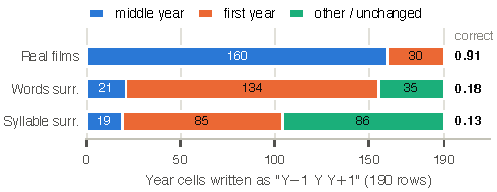
\includegraphics[width=\columnwidth]{figures/fig2_year_range.pdf}
  \caption{DeepSeek-V4-Pro's year repairs deteriorate after renaming, although all 190 year
  ranges are unchanged. Bars show the candidate written; the right panel shows repair accuracy.
  Taking the middle year matches 167 references (88\%).}
  \label{fig:year}
\end{figure}

\textbf{Year ranges retain useful candidates.} In the 190 source-style rows, the year is
``Y$-$1 Y Y$+$1'' and the middle candidate matches 167 references. This in-table rule is right
88\% of the time. DeepSeek is right 91\% on real films, but only 18\% on W and 13\% on S,
where it mostly chooses the first year (Figure~\ref{fig:year}). Unlike identifiers, the unchanged
year candidates retain a useful constraint after renaming, although the zero-shot prompt does
not state the rule. Lower repair thus reflects limited use of available evidence on unfamiliar
names. The other
commercial models show the same pattern: 171--176 correct years on O, versus 24--48 on
surrogates. Duration and genre repairs also decline after renaming; the rating-count formatting
rule behaves differently (Table~\ref{tab:moviescols}).

\begin{table}[t]
  \caption{Where knowledge acts on Movies: DeepSeek-V4-Pro repairs by column (repaired / errors).
  Identity columns are listed first; each condition uses its own error counts.}
  \label{tab:moviescols}
  \small
  \setlength{\tabcolsep}{4pt}
  \begin{tabular*}{\columnwidth}{@{\extracolsep{\fill}}lrrrr@{}}
    \toprule
    Column & O & F & W & S \\
    \midrule
    identifier & 78 / 190 & 75 / 190 & 0 / 190 & 0 / 190 \\
    title & 0 / 17 & 4 / 17 & 1 / 17 & 0 / 17 \\
    director & 18 / 43 & 27 / 39 & 7 / 43 & 2 / 43 \\
    writers & 1 / 129 & 27 / 125 & 3 / 129 & 1 / 129 \\
    \midrule
    year & 173 / 190 & 183 / 190 & 35 / 190 & 25 / 190 \\
    duration & 90 / 187 & 101 / 187 & 42 / 187 & 41 / 187 \\
    genre & 44 / 180 & 70 / 167 & 3 / 180 & 1 / 180 \\
    rating & 30 / 261 & 73 / 280 & 9 / 261 & 9 / 261 \\
    rating count & 2 / 768 & 26 / 1000 & 24 / 768 & 90 / 768 \\
    \bottomrule
  \end{tabular*}
\end{table}


\finding{Movies' commercial-model fresh--words gaps are $+$0.17--$+$0.42 at seed~0, with
surrogate identity repair F1 at most 0.05. Year repair also deteriorates despite retained
candidate evidence.}\label{find:movies}

\subsection{Beers: Formatting Errors}

Beers tests whether cleaners split city/state strings equally for real and fictitious names
(Table~\ref{tab:beers}). Seven models show no significant positive O\,$-$\,S effect; their
contrasts range from $-$0.08 to $+$0.04, with GPT's significant $-$0.03 in the opposite direction.
Qwen3.8-Max instead repairs 122 of 127 cities on O, 108 on W and 82 on S, giving a significant
total effect of $+$0.24. Its W-versus-S sign test has $p=0.019$ uncorrected and 0.15 after
correction over models. Dependence on familiar names therefore varies by model even for this
formatting repair. F is descriptive because its brewery concentration and alcohol distribution
differ from O (Section~\ref{sec:build-beers}).

\finding{Qwen3.8-Max has a positive total knowledge effect of $+$0.24 on Beers' formatting
errors; no significant positive effect appears in the other seven models.}\label{find:beers}

\begin{table}[t]
  \caption{Beers identity-column repair F1, O$-$S contrasts and repaired cities (O/F/W/S, of 127). $^\dagger$: Holm-corrected $p<0.05$ across eight O$-$S contrasts using entity/reply weights. F is descriptive; its brewery and alcohol-content distributions differ from O.}
  \label{tab:beers}
  \small
  \setlength{\tabcolsep}{3.5pt}
  \begin{tabular*}{\columnwidth}{@{\extracolsep{\fill}}lcccccr@{}}
    \toprule
    Model & O & F & W & S & O$-$S & Cities repaired \\
    \midrule
    DeepSeek-V4-Pro & 0.27 & 0.24 & 0.11 & 0.28 & $-$0.01 & 20 / 18 / 8 / 22 \\
    Qwen3.8-Max & 0.94 & 0.61 & 0.82 & 0.69 & +0.24$^\dagger$ & 122 / 67 / 108 / 82 \\
    GLM-5.3 & 0.94 & 0.88 & 0.89 & 0.94 & +0.00 & 120 / 110 / 116 / 117 \\
    GPT-6.1-Sol & 0.96 & 0.89 & 0.98 & 1.00 & $-$0.03 & 127 / 115 / 127 / 127 \\
    Qwen2.5-7B & 0.00 & 0.10 & 0.04 & 0.05 & $-$0.05 & 0 / 7 / 4 / 5 \\
    Llama-3.1-8B & 0.18 & 0.27 & 0.11 & 0.14 & +0.04 & 23 / 28 / 14 / 17 \\
    Qwen2.5-14B & 0.16 & 0.05 & 0.11 & 0.19 & $-$0.03 & 13 / 4 / 15 / 20 \\
    Qwen2.5-32B & 0.03 & 0.00 & 0.04 & 0.11 & $-$0.08 & 2 / 0 / 3 / 10 \\
    \bottomrule
  \end{tabular*}
\end{table}


\subsection{Stability over Construction Seeds}

Table~\ref{tab:seeds} reports construction variation separately from chunk-bootstrap intervals.
Hospital's total effect varies by at most 0.06 per model, and its spelling contrast by at most
0.05. F\,$-$\,W is more sensitive to the fresh error draw, with ranges reaching 0.11 for
DeepSeek and 0.13 for open models. Movies' commercial-model gaps remain positive across seeds,
including $+$0.39 to $+$0.44 for DeepSeek. The table gives the full model-specific ranges.

\begin{table}[t]
  \caption{Identity-column contrast ranges over three construction seeds; seed 0 is in
  Table~\ref{tab:main}. Fresh clean records are fixed while errors are redrawn.}
  \label{tab:seeds}
  \small
  \setlength{\tabcolsep}{2.5pt}
  \begin{tabular*}{\columnwidth}{@{\extracolsep{\fill}}l ccc cc@{}}
    \toprule
    & \multicolumn{3}{c}{Hospital} & \multicolumn{2}{c}{Movies} \\
    \cmidrule(lr){2-4}\cmidrule(l){5-6}
    Model & F$-$W & W$-$S & O$-$S & F$-$W & O$-$W \\
    \midrule
    DeepSeek & .34--.45 & .33--.36 & .66--.72 & .39--.44 & .31--.32 \\
    Qwen3.8 & .34--.38 & .33--.38 & .68--.69 & .38--.42 & .26--.28 \\
    GLM-5.3 & .28--.29 & .34--.37 & .57--.61 & .14--.19 & .07--.08 \\
    GPT-6.1 & .28--.29 & .09--.10 & .32--.34 & .32--.35 & .07 \\
    \midrule
    Qwen-7B & .16--.22 & .02--.07 & .19--.20 & .01--.03 & .00--.01 \\
    Llama-8B & .14--.24 & .01--.04 & .30 & .03--.04 & .03 \\
    Qwen-14B & .23--.31 & .12--.17 & .37--.42 & .03--.06 & .05 \\
    Qwen-32B & .17--.30 & .27--.28 & .49--.52 & .02--.03 & .01--.03 \\
    \bottomrule
  \end{tabular*}
\end{table}


\section{Does the Inflation Generalize?}\label{sec:generalize}

We test these contrasts against model scale, construction regularities, and added labels
or repeated records.

\begin{figure*}[t]
  \centering
  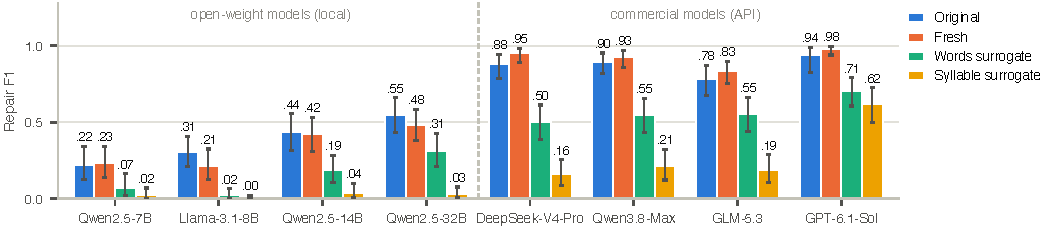
\includegraphics[width=\textwidth]{figures/fig6_scale.pdf}
  \caption{Hospital's total effect grows across Qwen2.5-7B/14B/32B, while S scores remain low.
  Identity-column repair F1, with Llama and commercial models for comparison; 95\% bootstrap
  intervals.}
  \label{fig:scale}
\end{figure*}

\subsection{Model Scale}\label{sec:scale}

Within Qwen2.5, Hospital's O\,$-$\,S grows from $+$0.20 at 7B to $+$0.40 at 14B and $+$0.52
at 32B, in the same order at every construction seed (Figure~\ref{fig:scale};
Table~\ref{tab:seeds}). S repair F1 stays low at 0.02, 0.04 and 0.03. Higher original scores
thus accompany a larger gap under entity replacement, with little improvement on unfamiliar
names in this family and benchmark.

\subsection{Recoverable Syllable Names}\label{sec:commercial}

GPT-6.1-Sol repairs 100 of Hospital S's 219 identity errors with 105 edits, compared with
28--37 repairs for the other commercial models. The constructor's 24-syllable inventory is
represented in every chunk and permits a
unique restoration for 95 corrupted names. GPT restores 74 of them; the other commercial models
restore 8--12 and open models at most one (Table~\ref{tab:decoding}). The inventory is used by
our analysis, not supplied to the cleaner. On digits, which it does not constrain, GPT repairs
6 of 97, like the others. This concentration is consistent with exploiting the restricted
vocabulary, linking GPT's stronger S performance to recoverable construction regularities.

\begin{table}[t]
  \caption{Hospital S repairs by recovery category. Unique and Ambig. use the 24-syllable inventory;
  Generic covers English terms, and Digits covers numeric tokens. Headers give cell counts, covering
  217 of 219 errors, with two address-spacing errors excluded from these counts.}
  \label{tab:decoding}
  \small
  \setlength{\tabcolsep}{4pt}
  \begin{tabular}{@{}lrrrr@{}}
    \toprule
    Model & Unique (95) & Ambig. (11) & Generic (14) & Digits (97) \\
    \midrule
    DeepSeek-V4-Pro & 8 & 0 & 13 & 5 \\
    Qwen3.8-Max & 12 & 0 & 12 & 11 \\
    GLM-5.3 & 10 & 0 & 12 & 8 \\
    GPT-6.1-Sol & 74 & 4 & 14 & 6 \\
    Open models & 0--1 & 0 & 0--3 & 0--6 \\
    \bottomrule
  \end{tabular}
\end{table}


\subsection{Labels, Error Positions and Repeated Records}\label{sec:labels}

The aligned setting adds labeled tuples and error positions without enlarging the main chunks.
The tuples provide examples of target values, while the positions identify which cells need
repair. DeepSeek-V4-Pro improves across conditions but retains
F\,$-$\,W gaps of $+$0.22 on Hospital and $+$0.58 on Movies (Figure~\ref{fig:aligned}).
Hospital's rounded W and S scores are only 0.01 apart. The extra information largely closes
the spelling contrast, while the advantage for real over surrogate entities remains.

\begin{figure}[tbp]
  \centering
  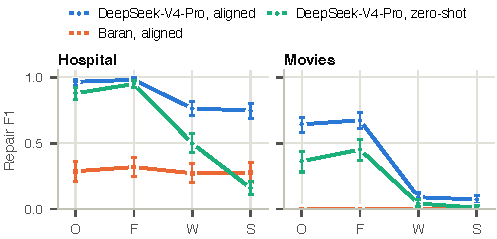
\includegraphics[width=\columnwidth]{figures/fig3_aligned.pdf}
  \caption{Labels and error positions improve DeepSeek-V4-Pro's repair but retain a fresh--words
  gap. Identity-column F1 in zero-shot and aligned settings; Baran is the aligned mean of three
  runs. Intervals are 95\% chunk-bootstrap intervals.}
  \label{fig:aligned}
\end{figure}

Baran with the same chunks, labels and positions scores 0.27--0.32 on Hospital and zero on
Movies identity columns. With whole-table perfect detection, it reaches 0.91--0.93 and
0.25--0.27, respectively, with little condition variation (Table~\ref{tab:aligned}). Whole-table access exposes
repeated records that can supply values missing from the main chunks. DeepSeek still leads Baran in every aligned Hospital and
Movies condition, but its advantage narrows on surrogates.

Table~\ref{tab:aligned} separates matched-chunk comparisons from whole-table results;
Figure~\ref{fig:aligned} plots the Hospital and Movies contrasts.

\begin{table}[t]
  \caption{Identity-column repair F1 under aligned and whole-table information. Aligned uses the same chunks,
  20 labeled tuples and error positions; Baran is the mean of three runs. Whole-table Baran
  uses perfect detection. TabClean uses DeepSeek-V4-Pro with development rows excluded.}
  \label{tab:aligned}
  \small
  \begin{tabular*}{\columnwidth}{@{\extracolsep{\fill}}l cccc@{}}
    \toprule
    Method & O & F & W & S \\
    \midrule
    \multicolumn{5}{@{}l}{\emph{Hospital}} \\
    \quad DeepSeek, aligned & 0.97 & 0.98 & 0.76 & 0.75 \\
    \quad Baran, aligned & 0.29 & 0.32 & 0.27 & 0.28 \\
    \quad Baran, whole table & 0.91 & 0.93 & 0.93 & 0.93 \\
    \quad TabClean & 1.00 & 1.00 & 0.96 & 0.99 \\
    \multicolumn{5}{@{}l}{\emph{Movies}} \\
    \quad DeepSeek, aligned & 0.64 & 0.67 & 0.09 & 0.07 \\
    \quad Baran, aligned & 0.00 & 0.00 & 0.00 & 0.00 \\
    \quad Baran, whole table & 0.27 & 0.26 & 0.26 & 0.25 \\
    \quad TabClean & 0.00 & 0.00 & 0.03 & 0.00 \\
    \multicolumn{5}{@{}l}{\emph{Beers}} \\
    \quad DeepSeek, aligned & 1.00 & 1.00 & 1.00 & 1.00 \\
    \quad Baran, aligned & 0.19 & 0.77 & 0.20 & 0.22 \\
    \quad Baran, whole table & 0.94 & 1.00 & 0.94 & 0.96 \\
    \quad TabClean & 1.00 & 1.00 & 1.00 & 1.00 \\
    \bottomrule
  \end{tabular*}
\end{table}


\subsection{Program-Generating Cleaner}\label{sec:e4}

TabClean~\cite{tabclean2026} writes cleaning programs rather than editing values directly.
With the settings in Section~\ref{sec:setup}, its identity-column F1 is 1.00, 1.00, 0.96 and
0.99 across Hospital O/F/W/S, 1.00 on Beers, and 0.00--0.03 on Movies
(Table~\ref{tab:aligned}). Its programs use repeated records and formatting rules; Movies'
source-specific identity values offer little such evidence. This offers an alternative to
direct value editing on the main chunks.

\finding{Labels and error positions improve DeepSeek-V4-Pro's repair without closing its
fresh--words gaps. Whole-table Baran and TabClean vary little across name replacements,
using repeated records and formatting rules to support repair.}\label{find:general}

\section{Knowledge Overrides the Table}\label{sec:conflict}

A familiar fact can conflict with a value the task requires preserving. We test which source
a cleaner follows by pairing familiar names with assigned values.

\subsection{Constructing Knowledge Conflicts}\label{sec:conflictdesign}

Starting from S, we assign target cells another real director or location in both dirty and
reference tables. Correctness here means preserving the assigned target, although other cells
in the row may still contain errors. Table~\ref{tab:conflictexample} illustrates the assignment
of Stanley Kubrick to \emph{Taken}, whose real director is Pierre Morel.

\begin{table}[t]
  \caption{A conflict target with the same assigned Director reference in three name versions.
  The real credit of \emph{Taken} (2008) is Pierre Morel; all other cells remain identical.}
  \label{tab:conflictexample}
  \small
  \begin{tabularx}{\columnwidth}{@{}lXll@{}}
    \toprule
    Version & Name & Year & Director \\
    \midrule
    Exact name & Taken & 2008 & Stanley Kubrick \\
    One-letter name & Takun & 2008 & Stanley Kubrick \\
    Surrogate control & Drikel Joujou & 2008 & Stanley Kubrick \\
    \bottomrule
  \end{tabularx}
\end{table}

Each target has an exact real name, a one-vowel-changed name and its syllable control. Only
the name differs across versions; attributes, other values, error positions and chunks are
fixed. Hospital and Beers receive internally consistent locations. Movies also updates
related director occurrences consistently, preventing another column from supplying the old
director as a candidate. The \companion{} specify these cross-column replacements.

The common pool contains 57 films, 24 hospitals and 48 breweries known to DeepSeek-V4-Pro.
Main chunks contain three targets and 17 other-entity fillers, with one row per target.
Supplementary Hospital/Beers conditions use three rows per target. Every model receives the
same pool, but rates use its own subset passing separate factual queries: 52--57 films,
22--24 hospitals and 7--48 breweries. Film knowledge accepts a credited full name or a surname
of at least four letters; location knowledge requires matching city and state. These are
conditional rates within the fixed pool.

The standard prompt asks for cleaning while preserving correct cells, without specifying
source priority. The \emph{table-evidence prompt} explicitly favors input-table evidence over
real-world knowledge. Both use the same chunks and known subsets.

\subsection{Measuring Rewrites}\label{sec:conflictmetric}

A directed rewrite changes the assigned Director or City to the paired entity's real-world
fact. Director outputs must contain a full credited name; cities must match the normalized
real city. The one-letter-name variant instead measures restoration of the exact real name.
These events are scored separately from any change to the target cell. Output parsing and
matching normalization are specified in the \companion{}.

Let $E_m$ contain entities passing model $m$'s factual queries, $s$ be target rows per entity,
and $z_{ej}$ indicate a matching rewrite in row $j$ of entity $e$. We report
\begin{equation*}
  \widehat{r}_m = \frac{1}{|E_m|}\sum_{e\in E_m}
                 \frac{1}{s}\sum_{j=1}^{s} z_{ej}.
\end{equation*}
For Movies, $s=1$, giving rewritten known films divided by known films. For $s=3$, row indicators
are first averaged within entities. Targets without a matching correction, including unusable
replies, remain in the denominator. Surrogate controls use the same known subset and paired
fact. Entity-bootstrap intervals follow Section~\ref{sec:setup}.

\begin{figure}[t]
  \centering
  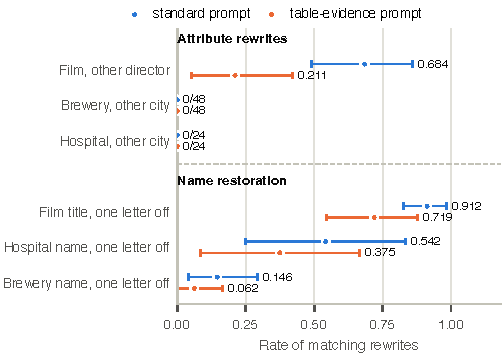
\includegraphics[width=\columnwidth]{figures/fig4_near_entity.pdf}
  \caption{DeepSeek-V4-Pro rewrites assigned directors more often than cities. Attribute rewrites
  and name restoration are separate events, using 57 films, 24 hospitals or 48 breweries with
  one row per target and 95\% entity-bootstrap intervals. Controls have zero directed rewrites.}
  \label{fig:near}
\end{figure}

\begin{figure}[t]
  \centering
  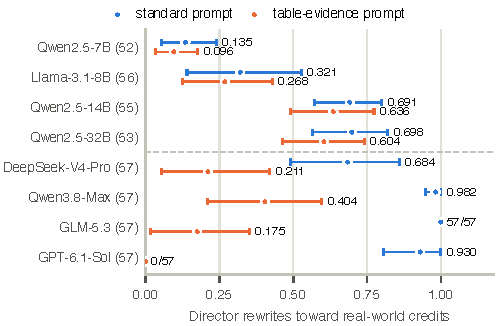
\includegraphics[width=\columnwidth]{figures/fig7_near_models.pdf}
  \caption{Table-evidence instructions reduce director rewrites unevenly. Rates divide
  matching real-credit rewrites by known films, with 95\% entity-bootstrap intervals.
  Parentheses give denominators, unchanged between prompts; Table~\ref{tab:conflictcounts}
  gives counts and control edits.}
  \label{fig:nearmodels}
\end{figure}

\subsection{Results}\label{sec:conflictresults}

\textbf{Familiar names draw factual rewrites.} Commercial models know the same 57 films and
rewrite 68\%--100\% of their assigned directors under the standard prompt
(Figure~\ref{fig:nearmodels}). DeepSeek, for example, rewrites 39/57. Controls also receive
Director edits, but none matches the paired film's real credit (Table~\ref{tab:conflictcounts}).
The paired names separate directed factual rewrites from other edits.

\begin{table}[t]
  \caption{Director rewrite counts among known films ($n/N$). Exact-name targets count edits
  matching a real-world director credit. Surrogate controls count any Director change;
  none matches the paired film's real credit.}
  \label{tab:conflictcounts}
  \small
  \setlength{\tabcolsep}{3pt}
  \begin{tabular*}{\columnwidth}{@{\extracolsep{\fill}}lrrrr@{}}
    \toprule
    & \multicolumn{2}{c}{Exact-name target} & \multicolumn{2}{c}{Surrogate control} \\
    \cmidrule(lr){2-3}\cmidrule(lr){4-5}
    Model & Standard & Evidence & Standard & Evidence \\
    \midrule
    DeepSeek-V4-Pro & 39/57 & 12/57 & 2/57 & 0/57 \\
    Qwen3.8-Max & 56/57 & 23/57 & 14/57 & 3/57 \\
    GLM-5.3 & 57/57 & 10/57 & 10/57 & 1/57 \\
    GPT-6.1-Sol & 53/57 & 0/57 & 7/57 & 0/57 \\
    Qwen2.5-7B & 7/52 & 5/52 & 0/52 & 0/52 \\
    Llama-3.1-8B & 18/56 & 15/56 & 2/56 & 2/56 \\
    Qwen2.5-14B & 38/55 & 35/55 & 2/55 & 0/55 \\
    Qwen2.5-32B & 37/53 & 32/53 & 0/53 & 0/53 \\
    \bottomrule
  \end{tabular*}
\end{table}


Within Qwen2.5, conditional rates rise from 0.135 at 7B to 0.691 at 14B and 0.698 at 32B.
Their known subsets differ, as shown in Table~\ref{tab:conflictcounts}. Llama knows 56 films
and rewrites 18 (0.321).

\textbf{The effect depends on the attribute.} Standard-prompt city rewrites reach at most
0.042 on Hospital and 0.140 on Beers across models. This is consistent with the distinction
between a particular directing credit and an institution that may operate at multiple locations.
DeepSeek also restores 91\% of one-letter-changed film names (Figure~\ref{fig:near}), a possible
spelling correction distinct from overriding an assigned attribute.

\textbf{Source-priority instructions help unevenly.} With the table-evidence prompt, GPT makes
no directed director rewrite (0/57). DeepSeek still rewrites 12 of 57 directors; GLM and
Qwen3.8-Max rewrite 10/57 and 23/57, respectively. Rates for Qwen2.5 at 14B and 32B remain
above 0.60 (Table~\ref{tab:conflictcounts}). These rewrites remain invalid under the prompt's
explicit table priority.

\finding{For known films, commercial models rewrite 68\%--100\% of assigned directors toward
real credits, while city rewrites are rare. Table-evidence instructions reduce their director
rates to 0.000--0.404, but Qwen2.5-14B/32B retain rates above 0.60.}\label{find:conflict}

\section{Benchmark Quality}\label{sec:quality}

The conflict test fixes values to preserve. We now examine whether reference-based scoring
rewards agreement with external fields or reproduction of the reference's own transformations.

\subsection{Systematic Reference Transformations}

Rayyan's audit pair has 1,000 rows and eleven columns, differing in 948 cells. Its
values exhibit patterns characteristic of spreadsheet conversion~\cite{ziemann2016gene}.
All 722 date differences map input \texttt{m/d/yy} to \texttt{d/int(yy)/mm}, with a two-digit
input month in the final position: for example, \texttt{1/1/13} becomes \texttt{1/13/01}.
Similarly, 31 of 32 pagination differences turn page ranges into month-name strings, such as
\texttt{70-6} to \texttt{Jun-70}.

\subsection{Stratified PubMed Checks}\label{sec:rayyan-audit}

We sample up to 80 cells per error type, including all volume/issue, pagination and ISSN
differences, for 279 cells. Automatic title matching selects the highest-similarity PubMed
candidate among up to five results at a normalized similarity of at least 0.9. This yields
152 matched cells associated with 121 PMIDs. The \companion{} give query construction,
normalization and retrieval provenance.

\textbf{Field-specific checks.} The date field \texttt{article\_jcreated\_at} is checked for
agreement with PubMed's publication year; the dataset does not document its exact semantics.
Volume and issue checks measure presence, using reference \texttt{-1} and dirty empty strings
as absence. Two reference volumes of \texttt{1}, for example, pass presence while differing
numerically from saved PubMed values \texttt{31} and \texttt{21}. Pagination matches the page
string, and ISSN accepts print or electronic identifiers. For encoding differences, a nonempty
set of reference-side changed words must all occur in the case-folded PubMed
word set, with accents retained. Encoding's dirty side is unassessed.

\begin{table}[tbp]
  \caption{Rayyan field checks: population $N_h$, sample $n_h$, title matches $m_h$,
  failed reference and passed dirty checks per matched cell. A dash denotes an unassessed dirty check.}
  \label{tab:rayyan}
  \small
  \setlength{\tabcolsep}{3pt}
  \begin{tabular*}{\columnwidth}{@{\extracolsep{\fill}}lrrrcc@{}}
    \toprule
    Check & $N_h$ & $n_h$ & $m_h$ & \shortstack{Reference fail\\$b_h/m_h$} & \shortstack{Dirty pass\\$d_h/m_h$} \\
    \midrule
    Year & 722 & 80 & 44 & 43/44 & 42/44 \\
    Changed words & 107 & 80 & 38 & 38/38 & --- \\
    Vol./issue & 75 & 75 & 46 & 28/46 & 17/46 \\
    Pages & 32 & 32 & 18 & 18/18 & 17/18 \\
    ISSN & 12 & 12 & 6 & 6/6 & 0/6 \\
    \bottomrule
  \end{tabular*}
\end{table}


Let $N_h$ be the error-cell population of type $h$, $m_h$ its title-matched count, and $b_h$
the matched references failing that field's check. The weighted reference-check failure rate is
\begin{equation}
  \widehat q = \sum_h \frac{N_h}{948}\frac{b_h}{m_h}.
  \label{eq:rayyan-weighted}
\end{equation}
Thus each within-type proportion uses matched cells, while weights follow the 948-cell audit
composition. The result is 95.2\% (95\% interval: 91.2--97.8\%;
Table~\ref{tab:rayyan}). Dates account for 722 of 948 error cells and
most of the weight. The interval conditions on the saved title matches and field checks;
matching uncertainty and dependence between cells sharing a PMID are outside this estimate.

\subsection{What the Reference Rewards}\label{sec:rayyan-rewards}

On the audit input, DeepSeek-V4-Pro's zero-shot output scores F1 0.002. For example, it changes
dirty ISSN \texttt{Mar-22} to \texttt{0003-3022}, matching the saved external ISSN, but the
reference is \texttt{22-Mar}. Scoring rejects this external match because the reference differs.

TabClean's distributed Rayyan input has 960 difference cells, rather than the audit's 948.
Both are 1,000-row, eleven-column tables with the same date-conversion pattern. We score the
archived output against its actual input pair and exclude 150 development rows. The remaining
850 rows contain 808 errors; 498 effective edits yield 461 credited repairs, giving
$F_1=2\times461/(498+808)=0.71$ after rounding. The \companion{} record the input-version
differences, development indices and saved output.

Of the 461 credited repairs, 434 (94\%) reproduce the reference date transformation. The
external field checks supply the complementary comparison: 42/44 matched dirty dates pass
the year check, whereas 43/44 references fail. Together, these cases show that reference matching
can reward conversion while denying credit to an identifier that matches the external record.

\subsection{Reference Issues in Other Benchmarks}

Hospital's reference places Helen Keller Memorial Hospital in Jefferson County, although its
city, Sheffield, is in Colbert County. Three commercial models correct some of these cells and
are penalized as false edits. These smaller issues illustrate the same distinction between
reference agreement and external correctness. The \companion{} give their counts and an
example of duplicate writer credits in Movies.

\finding{Rayyan's systematic date and page conversions affect repair credit. Stratified field
checks against title-matched PubMed records give 95.2\% weighted reference-check failure
(95\% interval: 91.2--97.8\%), using the 948-cell type composition. On TabClean's version,
434/461 credited repairs (94\%), after excluding 150 development rows, reproduce the reference
date transformation.}\label{find:quality}

\section{Lessons and Recommendations}\label{sec:discussion}

Our results suggest the following evaluation practices.

\textbf{Report familiarity alongside repair performance.} Evaluate original and paired name
surrogates, using both word and syllable names to distinguish their roles
(Findings~\ref{find:hospital}--\ref{find:beers}). Fresh real records address a different question:
refreshing rows leaves knowledge of familiar entities available. These contrasts play
complementary roles in interpreting repair performance.

\textbf{Relate expectations to recovery evidence.} Group errors by the information retained
in the shown input, rather than relying on one aggregate benchmark score. Candidate rules,
source-specific values and underdetermined identifiers require different interpretations
(Section~\ref{sec:recoverability}). Cleaners can use local rules or supporting records where
they are available, and distinguish finding an error from supplying its value.

\textbf{Equalize information in method comparisons.} State which labels, error positions and
repeated records each method receives. Compare aligned settings before interpreting differences
between chunk-based and whole-table cleaners (Finding~\ref{find:general}).

\textbf{Set source priority and test value preservation.} Resolving Movies' source conflicts
requires selecting the benchmark's preferred values. The conflict test instead requires
preserving an assigned director. Evaluate repair and preservation under that priority,
distinguishing directed factual rewrites from other edits (Finding~\ref{find:conflict}).

\textbf{Check what reference matching rewards.} Compare reference fields with independent
records under explicit criteria (Finding~\ref{find:quality}). Conversion patterns explain
credited changes, while input versions and development exclusions identify the scored values.

\subsection{Applying \core{} to Other Benchmarks}\label{sec:apply}

Adapting \core{} leaves the cleaner unchanged but requires an error profile, a compatible fresh
source, two naming styles and acceptance checks. Profiling identifies the available recovery
evidence and the intended target, including source priorities and reference transformations.
The \companion{} provide an application guide. Matching and imputation offer future settings.

\subsection{Artifact and Result Replay}\label{sec:artifact}

The statistical core supports offline replay of the condition contrasts, conflict rates and
Rayyan checks. It provides Hospital/Beers tables and archived evidence; Movies uses numerical
witnesses and saved continuation summaries. A separate authorized local entry checks historical
movie inputs, replies and scoring-code hashes before re-scoring. The \companion{} map C1--C3
to their input versions, executable entries and reported results, distinguishing public numerical
replay from reader-supplied row-level validation.

\subsection{Limitations}\label{sec:limitations}

The datasets diagnose recovery mechanisms and reference transformations in entity-rich public
tables, rather than estimate their prevalence across cleaning workloads. Transfer to private data
also depends on size, sparsity, task complexity and the availability of supporting records.
Our comparisons change name forms as well as familiarity,
and F introduces record-difficulty differences (Table~\ref{tab:conditions}). Beers F has
different brewery concentration and alcohol distributions, while Hospital's restricted syllables
provide the regularity observed for GPT (Section~\ref{sec:commercial}). The study covers eight
commercial and open-weight cleaners on English tables concerning mainly US entities, with decoding differences stated
in Section~\ref{sec:setup}; it does not cover Claude or Gemini.

Intervals summarize fixed constructions and archived replies, rather than repeated API calls.
Chunk resampling does not separately estimate dependence between chunks sharing an entity;
entity resampling in the conflict test leaves shared-chunk dependence outside its uncertainty
estimate. The controlled conflict measures source priority, not the prevalence of conflicting
values in private data. Whole-table results show how additional records can supply evidence
absent from the main chunks.

\section{Conclusion}\label{sec:conclusion}

\core{} connects the evidence used to recover values with the targets that determine
preservation and repair credit. Paired entity replacements and fresh records test recovery
from familiar and unfamiliar inputs. Across eight LLMs, familiar
entities contribute substantially to Hospital's identity-column scores and to Movies scores for
commercial models. The continuation probe finds no positive evidence of benchmark-row memorization in the
tested models. Direct editing and table-based repair draw on different evidence, so
information access also shapes these effects.

Recovery alone does not determine whether an edit serves the task. Models can replace assigned
directors with familiar real credits, with uneven reductions under table-evidence instructions.
Repair credit ultimately depends on the reference. Rayyan's stratified field checks and
credited date conversions show how a reference can reward its own transformations.
Evaluations should therefore connect recovery on unfamiliar entities with source-priority
and value-preservation tests, and inspect the targets used to score repairs. The construction
principles provide a basis for studying these questions in other entity-based data preparation tasks.

\bibliographystyle{ACM-Reference-Format}
\bibliography{refs}

\end{document}
